\documentclass{article}    
\usepackage[letterpaper,margin=1in]{geometry}
\usepackage{lastpage}
\usepackage{graphicx}
\usepackage{fancyhdr}
\usepackage{enumitem}
\usepackage{amssymb}

\fancypagestyle{plain}{%
\fancyhf{}%
\lhead{ECS165A SQ18}
\rhead{\today}
\cfoot{Homework 2\\ \thepage\ of \pageref{LastPage} }
\renewcommand{\headrulewidth}{0.4pt}
\renewcommand{\footrulewidth}{0.4pt}
}

\pagestyle{fancy}
\fancyhf{}
\lhead{ECS165A SQ18}
\rhead{\today}
\cfoot{Homework 2\\ \thepage\ of \pageref{LastPage} }
\renewcommand{\headrulewidth}{0.4pt}
\renewcommand{\footrulewidth}{0.4pt}

\begin{document}

\title{Homework 2}
\author{Name: Shivang Soni\\SID: 915623718}

\maketitle

Due 11:59PM May 2, 2018. {\bf READ ALL DIRECTIONS VERY CAREFULLY!} 
Submit your tex files along with a generated PDF.
You {\bf MUST} put each problem on a separate page with 1a on the first page, for example 1a will be on page 1 and 1b will be on page 2 (this template is already setup for this). Try to keep each answer to one page. 
You {\bf MUST} put your name and student ID in the provided author section above. {\bf FAILURE TO DO SO MAY RESULT IN NO CREDIT!} 


\section*{Problem 1}
For this problem you will consider following relation and set of FDs:\\
$R(A,B,C,D,E)$\\
$B\rightarrow C$\\
$BE\rightarrow D$\\
$DC\rightarrow E$\\
$DE\rightarrow A$\\

\begin{enumerate}[label=\alph*.]
\item What are the keys of $R$? {\bf (Show your closures)} \\
{\bf % Problem 1a goes below

$\{B\}^+ = \{ B,C\}$ \\
$\{A\}^+ = \{ A\}$ \\
$\{C\}^+ = \{ C\}$ \\
$\{D\}^+ = \{ D\}$ \\
$\{E\}^+ = \{ E\}$ \\
$\{AB\}^+ = \{A,B,C\}$ \\
$\{AC\}^+ = \{ A,C\}$ \\
$\{AD\}^+ = \{A,D\}$ \\
$\{AE\}^+ = \{ A,E\}$ \\
$\{BC\}^+ = \{B,D\}$ \\
Key:$\{BD\}^+ = \{ B,C,D,E,A\}$ \\
Key:$\{BE\}^+ = \{B,C,D,E,A\}$ \\
$\{CD\}^+ = \{ C,D,E,A\}$ \\
$\{CE\}^+ = \{ C,E\}$ \\
$\{DE\}^+ = \{ D,E,A\}$ \\

Hence from the above closure the Keys of the relation R is $\{B,D\}$ and $\{B,E\}$ } \clearpage
\item Show that the set of FDs is a minimal basis; if it is not a minimal basis find a minimal basis for the FDs.\\
{\bf % Problem 1b goes below
. \\ \\ \\
$\{B\}^+ = \{ B\}$ \\
$\{B,E\}^+ = \{ C,B,E\}$ \\
$\{D,C\}^+ = \{ D,C\}$ \\
$\{D,E\}^+ = \{ D,E\}$ \\ \\

Try to remove the attributes from the functional dependencies and make sure if the RHS attribute can be reached. \\ \\ \\

From the relation $BE -> D$\\
Try removing E$\{B\}^+ = \{B,C\}$ \\
Try removing B$\{E\}^+ = \{ E\}$ \\ \\ \\
Similarly, From the relation $DC -> E$\\
Try removing D$\{C\}^+ = \{C\}$ \\
Try removing C$\{D\}^+ = \{ D\}$ \\ \\ \\

and also From the relation $DE -> A$\\
Try removing D$\{E\}^+ = \{E\}$ \\
Try removing E$\{D\}^+ = \{D\}$ \\

Means the FD's is a minimal basis.
 } \clearpage
\item What are all of the BCNF violations that follow from the FDs? {\bf (Don't just consider the listed FDs, but all that follow.)} \\
{\bf % Problem 1c goes below
R(A,B,C,D,E)\\
$B \rightarrow C$\\
$BE \rightarrow D$\\
$DC \rightarrow E$\\
$DE \rightarrow A$\\


For the above set of the functional dependencies the FD's that voilets are: \\ 
$B \rightarrow C$\\
$DC \rightarrow E$\\
$DE \rightarrow A$\\

now we must also consider all the functional dependencies that follows those listed above.\\

For FD $B \rightarrow C$ find closure of the FD's that follows\\
$\{AB\}^+ = \{ A,B,C\}$  --> this is a voilation\\
$\{BE\}^+ = \{ A,B,C,D,E\}$ \\
$\{BD\}^+ = \{ A,B,C,D,E\}$ \\

thus $AB \rightarrow C$ FD also voilates BCNF \\

For FD $DC \rightarrow E$ find closure of the FD's that follows\\
$\{ACD\}^+ = \{ A,D,C,E\}$  --> this is a voilation\\
$\{BCD\}^+ = \{ A,D,C,E,B\}$

thus $ACD \rightarrow E$ FD also voilates BCNF \\




For FD $DE \rightarrow A$ find closure of the FD's that follows\\
$\{CDE\}^+ = \{ A,D,C,E\}$  --> this is a voilation\\
$\{BCD\}^+ = \{ A,D,C,E,B\}$

thus $CDE \rightarrow A$ FD also voilates BCNF \\

All the functional dependencies with the voilations are:\\
$CDE \rightarrow A$\\
$ACD \rightarrow E$\\
$AB \rightarrow C$\\
$B \rightarrow C$\\
$DC \rightarrow E$\\
$DE \rightarrow A$\\
$CD \rightarrow A$\\
 } \clearpage
\item Decompose $R$ into BCNF. For each relation, list the keys, and make sure the set of FDs for each is a minimal basis.\\
{\bf % Problem 1d goes below
Relation is:\\
$B \rightarrow C$\\
$BE \rightarrow D$\\
$DC \rightarrow E$\\
$DE \rightarrow A$\\ \\ \\

Based on the voilators above we decomose the relation as \\ \\

Considering FD $B->C$ for decomposition \\
R1(B,C)\\
$B  \rightarrow C$\\ \\

In Relation R1 B is a key i.e. $\{B\}^+ = \{ B,C\}$ means all attribute in relation R1 is attained\\ \\
R2(A,B,D,E)\\
$BE \rightarrow D$\\
$DE \rightarrow A$\\

As In Relation R2 there is only 1 key \{B,E\} so we need to decompose the relation based on the functional dependency that violates.\\ \\

R3(A,D,E)\\
$DE \rightarrow A$\\


In Relation R3 DE is a key i.e. $\{DE\}^+ = \{ D,E,A\}$ means all attribute in relation R3 is attained\\ \\

R4(B,D,E)\\
$BE \rightarrow D$\\

In Relation R4 BE is a key i.e. $\{BE\}^+ = \{ B,E,D\}$ means all attribute in relation R4 is attained\\ \\


After Decomposing R into BCNF the relations we obtained are R1,R3,R4 \\

 } \clearpage
\item What are all of the 3NF violations that follow from the FDs? {\bf (Don't just consider the listed FDs, but all that follow.)} \\
{\bf % Problem 1e goes below

R(A,B,C,D,E)\\
$B \rightarrow C$\\
$BE \rightarrow D$\\
$DC \rightarrow E$\\
$DE \rightarrow A$\\

The functional dependencies which voilates are:\\

$B \rightarrow C$\\
$DE \rightarrow A$\\

and $DC \rightarrow E$ is not a voilator of 3NF as its RHS i.e. E is a prime attribute. \{BE\} is the key for the above relation\\

now other then these functional dependencies the functional dependencies that follows are:\\

For FD $B \rightarrow C$ find closure of the FD's that follows\\
$\{AB\}^+ = \{ A,B,C\}$  --> this is a voilation\\
$\{BE\}^+ = \{ A,B,C,D,E\}$ \\
$\{BD\}^+ = \{ A,B,C,D,E\}$ \\

thus $AB \rightarrow C$ FD also voilates 3NF \\

For FD $DE \rightarrow A$ find closure of the FD's that follows\\
$\{CDE\}^+ = \{ A,D,C,E\}$  --> this is a voilation\\
$\{BCD\}^+ = \{ A,D,C,E,B\}$

thus $CDE \rightarrow A$ FD also voilates 3NF \\


All the functional dependencies with the voilations are:\\
$CDE \rightarrow A$\\
$AB \rightarrow C$\\
$B \rightarrow C$\\
$DE \rightarrow A$\\ } \clearpage
\item Decompose $R$ into 3NF. For each relation, list the keys, and make sure the set of FDs for each is a minimal basis. \\
{\bf % Problem 1f goes below

As all the FD's dependencies for the relation R is a minimal basis \\

Now for decomposition all the Relation must include all FD's and also Relation having Super Key in it\\

As well as we can remove the relation if it is the subset of another relation \\ 

R1(B,C)   R2(B,D,E)  R3(D,C,E)  R4(A,D,E) \\ \\

As no relation is a subset of another relation so we don't remove and no other relation will be added as R2 is the Super Key of the relation R.



 } \clearpage
\item What are all of the 4NF MVD violations that follow from the FDs? \\
{\bf % Problem 1g goes below
% Use $\twoheadrightarrow$ for MVDs

Firstly taking into account the functional dependencies that voilates BCNF are: \\ \\

$B \rightarrow C$ \\
$DC \rightarrow E$ \\
$DE \rightarrow A$ \\
$AB \rightarrow C$ \\
$ACD \rightarrow E$\\
$CDE \rightarrow A$\\
Now For these FD's Corrosponding MVD's are:\\ \\
These are the MVD voilations that follow from the FD's.

Step 1:\\
Apply promotion to the FD's that voilates BCNF \\
$B \twoheadrightarrow C$\\
$DC \twoheadrightarrow E$ \\
$DE \twoheadrightarrow A$ \\ 
$AB \twoheadrightarrow C$ \\ 
$ACD \twoheadrightarrow E$\\
$CDE \twoheadrightarrow A$\\ \\
Step 2:\\
Apply Complement \\
$B \twoheadrightarrow ADE$\\
$DC \twoheadrightarrow AB$ \\
$DE \twoheadrightarrow BC$ \\
$AB \twoheadrightarrow DE$ \\
$ACD \twoheadrightarrow B$ \\
$CDE \twoheadrightarrow B$ \\ \\

Above are all the MVD voilations that follow from the FDs\\ \\





 } \clearpage
\item Decompose $R$ into 4NF. For each relation, list the keys, FDs and MVDs. \\
{\bf % Problem 1h goes below
 R1(B,C) \\
 $B \rightarrow C$\\
 $B \twoheadrightarrow C$\\
 here in the above relation B is a key \\ \\
 
 R2(A,B,D,E) \\ 
 $BE \rightarrow D$\\
 $DE \rightarrow A$\\
 $BE \twoheadrightarrow D$\\
 $DE \twoheadrightarrow A$\\
 $BE \twoheadrightarrow A$\\
 $DE \twoheadrightarrow B$\\
 here key is BE as its closure gives all the attributes present in relation R2\\ \\
 
 As from the relation R2 we have violation for all other FD's except BE is we will decompose R2\\ \\
 
 R3(A,D,E)\\
 $DE \rightarrow A$\\
 $DE \twoheadrightarrow A$\\ \\
 
 Here DE is the key for relation R3.\\ 
 
 R4(E,D,B)\\
 $BE \rightarrow D$\\
 $BE \twoheadrightarrow D$\\ \\
 Here BE is the key for relation R3.\\
 
 The relations after decomposition are as follows:\\ R1(B,C) R3(A,D,E) R4(E,D,B) } \clearpage
\item If you project the relation $R$ onto $S(A,B,C)$ what nontrivial FDs and MVDs hold in $S$? \\
{\bf % Problem 1i goes below
. \\ \\
The functional dependencies are:\\
$B \rightarrow C$\\
$BE \rightarrow D$\\
$DC \rightarrow E$\\
$DE \rightarrow A$\\

Closure of the relation R onto S(A,B,C)\\
$\{B\}^+ = \{ B,C\}$ \\
$\{A\}^+ = \{ A\}$ \\
$\{C\}^+ = \{ C\}$ \\
$\{A,B\}^+ = \{ B,C,A\}$ \\
$\{A,C\}^+ = \{ A,C\}$ \\
$\{B,C\}^+ = \{ B,C\}$ \\


The new FD's which are produced by the relation are:\\
$AB \rightarrow C$\\
$AB \twoheadrightarrow C$
 } \clearpage
\end{enumerate}

\section*{Problem 2} 
For this problem you will consider following relation and set of FDs:\\
$Courses(C,T,I,H,R,S,G)$\\
$CT\rightarrow I$\\
$TIH\rightarrow R$\\
$THR\rightarrow C$\\
$THS\rightarrow R$\\
$CTS\rightarrow G$\\

Where $C, T, I, H, R, S,$ and $G$ are the course, term, instructor, hour, room, student, and grade respectively. \\

\begin{enumerate}[label=\alph*.]
\item Use the chase test to prove/disprove that  $CTH\rightarrow G$ holds in Courses.\\
{\bf % Problem 2a goes below
% Below is an example of the tables & and applying of FDs
%\begin{tabular}{ c | c | c | c | c | c | c }
%  $A$ & $B$ & $C$ & $D$ & $E$ & $F$ & $G$ \\ 
%  \hline\hline
%  $a$ & $b$ & $c_1$ & $d$ & $e_1$ & $f_1$ & $g$\\
%  \hline 
%  $a$ & $b$ & $c_2$ & $d$ & $e_2$ & $f_2$ & $g_2$\\
%\end{tabular}
%
%Apply $AB\rightarrow C$
%
%\begin{tabular}{ c | c | c | c | c | c | c }
%  $A$ & $B$ & $C$ & $D$ & $E$ & $F$ & $G$ \\ 
%  \hline\hline
%  $a$ & $b$ & $c_1$ & $d$ & $e_1$ & $f_1$ & $g$\\
%  \hline 
%  $a$ & $b$ & $c_1$ & $d$ & $e_2$ & $f_2$ & $g_2$\\
%\end{tabular}

\begin{tabular}{ c | c | c | c | c | c | c }
  $C$ & $T$ & $I$ & $H$ & $R$ & $S$ & $G$ \\ 
  \hline\hline
  $c$ & $t$ & $i_1$ & $h$ & $r_1$ & $s_1$ & $g$\\
  \hline 
  $c$ & $t$ & $i_2$ & $h$ & $r_2$ & $s_2$ & $g_2$\\
\end{tabular}

Apply $CT \rightarrow I$ FD we get:\\

\begin{tabular}{ c | c | c | c | c | c | c }
  $C$ & $T$ & $I$ & $H$ & $R$ & $S$ & $G$ \\ 
  \hline\hline
  $c$ & $t$ & $i_1$ & $h$ & $r_1$ & $s_1$ & $g$\\
  \hline 
  $c$ & $t$ & $i_1$ & $h$ & $r_2$ & $s_2$ & $g_2$\\
\end{tabular}

Apply $TIH \rightarrow R$ FD we get:\\

\begin{tabular}{ c | c | c | c | c | c | c }
  $C$ & $T$ & $I$ & $H$ & $R$ & $S$ & $G$ \\ 
  \hline\hline
  $c$ & $t$ & $i_1$ & $h$ & $r_1$ & $s_1$ & $g$\\
  \hline 
  $c$ & $t$ & $i_1$ & $h$ & $r_1$ & $s_2$ & $g_2$\\
\end{tabular}


Thus Chase test fails to prove that the dependency $CTH \rightarrow G$ holds in Courses } \clearpage
\item Use the chase test to prove/disprove that  $CTH\rightarrow R$ holds in Courses.\\
{\bf % Problem 2b goes below


\begin{tabular}{ c | c | c | c | c | c | c }
  $C$ & $T$ & $I$ & $H$ & $R$ & $S$ & $G$ \\ 
  \hline\hline
  $c$ & $t$ & $i_1$ & $h$ & $r_1$ & $s_1$ & $g$\\
  \hline 
  $c$ & $t$ & $i_2$ & $h$ & $r_2$ & $s_2$ & $g_2$\\
\end{tabular}

Apply $CT \rightarrow I$ FD we get:\\

\begin{tabular}{ c | c | c | c | c | c | c }
  $C$ & $T$ & $I$ & $H$ & $R$ & $S$ & $G$ \\ 
  \hline\hline
  $c$ & $t$ & $i_1$ & $h$ & $r_1$ & $s_1$ & $g$\\
  \hline 
  $c$ & $t$ & $i_1$ & $h$ & $r_2$ & $s_2$ & $g_2$\\
\end{tabular}

Apply $TIH \rightarrow R$ FD we get:\\

\begin{tabular}{ c | c | c | c | c | c | c }
  $C$ & $T$ & $I$ & $H$ & $R$ & $S$ & $G$ \\ 
  \hline\hline
  $c$ & $t$ & $i_1$ & $h$ & $r_1$ & $s_1$ & $g$\\
  \hline 
  $c$ & $t$ & $i_1$ & $h$ & $r_1$ & $s_2$ & $g_2$\\
\end{tabular}


Thus Chase test  proved that the dependency $CTH \rightarrow R$ holds in Courses } \clearpage
\item Use the chase test to prove/disprove that the proposed decomposition has a lossless join.\\
$R_1(C, T, I, H)$\\
$R_2(C, T, H, R, S)$\\
$R_3(C, T, S, G)$\\
{\bf % Problem 2c goes below

R1(C,T,I,H)\\
$CT \rightarrow I$\\ \\

R2(C,T,H,R,S)\\
$THR \rightarrow C$\\
$THS \rightarrow R$\\ \\

R3(C,T,S,G)\\
$CTS \rightarrow G$ \\ \\ \\ 

\begin{tabular}{ c | c | c | c | c | c | c }
  $C$ & $T$ & $I$ & $H$ & $R$ & $S$ & $G$ \\ 
  \hline\hline
  $c$ & $t$ & $i$ & $h$ & $r_1$ & $s_1$ & $g_1$\\
  \hline 
  $c$ & $t$ & $i_2$ & $h$ & $r$ & $s$ & $g_2$\\
  \hline 
  $c$ & $t$ & $i_3$ & $h_3$ & $r_3$ & $s$ & $g$\\
\end{tabular} \\

Apply $CT \rightarrow I$ on relation R1 and R2 we get:\\

\begin{tabular}{ c | c | c | c | c | c | c }
  $C$ & $T$ & $I$ & $H$ & $R$ & $S$ & $G$ \\ 
  \hline\hline
  $c$ & $t$ & $i$ & $h$ & $r_1$ & $s_1$ & $g_1$\\
  \hline 
  $c$ & $t$ & $i$ & $h$ & $r$ & $s$ & $g_2$\\
  \hline 
  $c$ & $t$ & $i_3$ & $h_3$ & $r_3$ & $s$ & $g$\\
\end{tabular} \\ \\
Apply $THS \rightarrow R$ on relation R2 and R3 we get:\\

\begin{tabular}{ c | c | c | c | c | c | c }
  $C$ & $T$ & $I$ & $H$ & $R$ & $S$ & $G$ \\ 
  \hline\hline
  $c$ & $t$ & $i$ & $h$ & $r_1$ & $s_1$ & $g_1$\\
  \hline 
  $c$ & $t$ & $i$ & $h$ & $r$ & $s$ & $g_2$\\
  \hline 
  $c$ & $t$ & $i_3$ & $h_3$ & $r$ & $s$ & $g$\\
\end{tabular} \\

Apply $CTS \rightarrow G$ on relation R2 and R3 we get:\\

\begin{tabular}{ c | c | c | c | c | c | c }
  $C$ & $T$ & $I$ & $H$ & $R$ & $S$ & $G$ \\ 
  \hline\hline
  $c$ & $t$ & $i$ & $h$ & $r_1$ & $s_1$ & $g_1$\\
  \hline 
  $c$ & $t$ & $i$ & $h$ & $r$ & $s$ & $g$\\
  \hline 
  $c$ & $t$ & $i_3$ & $h_3$ & $r$ & $s$ & $g$\\
\end{tabular} \\


Thus Chase test  prove that proposed decomposition has lossless join\\ } \clearpage
\item Decompose Courses into 3NF.\\
{\bf % Problem 2d goes below
Functional dependencies for the relation are:\\
$CT \rightarrow I$\\
$TIH \rightarrow R$\\
$THS \rightarrow R$\\
$THR \rightarrow C$\\
$CTS \rightarrow G$\\

for 3 NF decomposition we require:\\
1.) Check to see if the FD's are in minimum basis\\
2.) Left side is a super key or right side has prime attribute\\
3.) Add all the FD's into the relation\\
4.) Add the relation into 3NF if the current relations does not have super key and remove if any relation is the subset of another relation\\

There are 2 FD's which does not voilates 3NF i.e.\\ 
$TIH \rightarrow R$\\
$THS \rightarrow R$\\

All the FD's are minimal basis.\\ \\

Key for the relation:\\
$\{CT\}^+ = \{ C,T,I\}$ \\
super key: $\{THS\}^+ = \{ T,H,S,C,R,G,I\}$ \\
$\{THR\}^+ = \{ T,H,R,C,I,G\}$ \\
$\{CTS\}^+ = \{ C,T,S,G,I\}$ \\

R1(C,T,I)\\
$CT \rightarrow I$\\ \\
R2(T,I,H,R)\\
$TIH \rightarrow R$\\ \\
R3(T,H,S,R)\\
$THS \rightarrow R$\\ \\
R4(T,H,R,C)\\ 
$THR \rightarrow C$\\ \\
R5(C,T,S,G)\\
$CTS \rightarrow G$\\


So all the relations R1,R2,R3,R4,R5 are in 3NF. } \clearpage
\item Which of your relations in 3NF are not in BCNF?\\
{\bf % Problem 2e goes below

The relations which are in BCNF is just:\\
$THS \rightarrow R$\\
other then the above relation all other relations violates BCNF\\

4 relations that violates are:\\
$CT \rightarrow I$\\
$TIH \rightarrow R$\\
$THR \rightarrow C$\\
$CTS \rightarrow G$\\

now the relations are like:\\
R1(C,T,I)\\
$CT \rightarrow I$\\ 
No FD voilates for this relation \\ 

R2(C,T,H,R,S,G)\\
$THR \rightarrow C$\\
$CTS \rightarrow G$\\
$THS \rightarrow R$\\ 
Two FD's voilates for this relation i.e. \\
$THR \rightarrow C$\\
$CTS \rightarrow G$\\
Decompose R2 into relation R3 and R4\\ 

R3(C,T,S,G)\\
$CTS \rightarrow G$\\ 
No FD voilates for this relation \\ 


R4(C,T,S,H,R)\\
$THR \rightarrow C$\\
$THS \rightarrow R$\\ 
1 FD's voilates for this relation i.e. \\
$THR \rightarrow C$\\
Decompose R4 into relation R5 and R6\\ 


R5(T,H,R,C)\\
$THR \rightarrow C$\\ 
No FD voilates for this relation \\ 

R3(T,H,R,S)\\
$THS \rightarrow R$\\ 
No FD voilates for this relation \\ \\

For BCNF R1,R3,R5,R6 holds.

The relation which is in 3NF but not in BCNF is 
R2(T,I,H,R)\\
$TIH \rightarrow R$\\ \\ } \clearpage
\item Which of your relations in 3NF are not in 4NF?\\
{\bf % Problem 2f goes below
The below relation holds in 3NF:\\ \\
R1(C,T,I)\\
$CT \rightarrow I$\\ 
R2(T,I,H,R)\\
$TIH \rightarrow R$\\ 
R3(T,H,S,R)\\
$THS \rightarrow R$\\ 
R4(T,H,R,C)\\ 
$THR \rightarrow C$\\ 
R5(C,T,S,G)\\
$CTS \rightarrow G$\\

4NF MVD's are :\\
R1(C,T,I):\\
$CT \rightarrow I$\\
$CT \twoheadrightarrow I$\\

R2(C,T,H,R,S,G):\\
$CTS \rightarrow G$\\
$THS \rightarrow R$\\
$THR \rightarrow C$\\
$CTS \twoheadrightarrow G$\\
$THS \twoheadrightarrow R$\\
$THR \twoheadrightarrow C$\\

as THS is the key so other MVD's voilates decompose R2

R3(T,C,S,G):\\
$CTS \rightarrow G$\\

R4(T,C,S,H,R):\\
$THS \twoheadrightarrow R$\\
$THR \twoheadrightarrow C$\\
$THS \rightarrow R$\\
$THR \rightarrow C$\\
decompose R4 to R5 and R6\\

R5(T,H,R,C):\\
$THR \twoheadrightarrow C$\\

R6(T,H,R,S):\\
$THS \twoheadrightarrow R$\\


So the 3NF relation not in 4NF is:\\
R2(T,I,H,R),R3(T,H,S,R),R5(C,T,S,G) \\ 
The relation which is in 3NF but not in 4NF is\\ 
R2(T,I,H,R)\\
$TIH \rightarrow R$\\ \\ } \clearpage
\end{enumerate}

\section*{Problem 3}
Design a academic genealogy database with one entity set: Academics. An academic's
academic parent is their doctoral advisor, their grandparent is their doctoral
advisor's advisor, etc. There are at least two other signators on a disertation
other than the doctoral advisor. The information to record about academics 
includes their birth name, date of birth, date of death (if deceased), field, 
dissertation title, institution, doctoral advisor, second signer, third signer
and any academic children.\\
{\bf % Problem 3 goes below
% Use \includegraphics as shown below to include an image
%\includegraphics{Image.png}

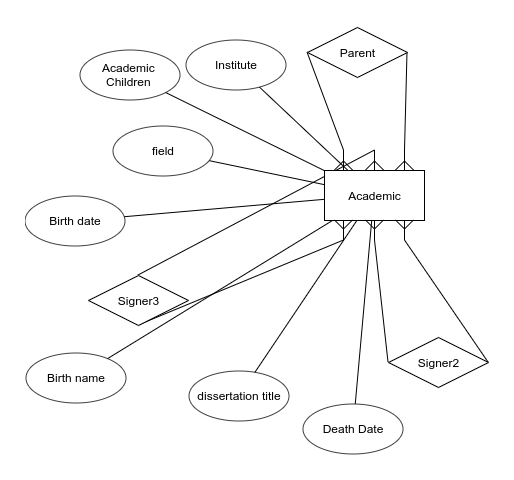
\includegraphics{erdplus-diagram.png} } \clearpage 

\end{document}